\chapter{Energy Landscape Software Library}
\label{ch:software}
\graphicspath{{software/fig/}}
In this chapter, we discuss the aims and structure of the energy landscape library `ELLib', which has been developed in order to study large and versatile systems.
We detail the various potentials and methods that have been included in the library and how they have parallelised.
Finally, there is a demonstration of the library being applied to a structural optimisation problem.

The software library and the program used for the structural optimisation are both accessible in the supplementary materials, detailed in \cref{ch:appendix}.
Alternatively, the most up-to-date version of `ELLib' is available on GitHub at the link: \url{https://github.com/sjavis/ellib}.
This chapter provides details about how it can be used and will be further developed into comprehensive documentation in the near future.


\section{Software structure}
The energy landscape software is contained within an object-oriented C++ library that can be imported and run inside a user script or as a part of another program.
It has been designed in a modular manner so that different methods and applications can be easily interchanged and new methods can be implemented without difficulty.

At the core of almost all energy landscape methods is some form of energy minimisation, often with modifications, therefore ELLib contains a sub-library specifically for the minimisation methods.
Outside of this are the landscape exploration methods which make use of the minimisation, such as pathway and transition state search.
However, there is not always a clear division between the minimisation methods and the landscape methods.
For example, the genetic algorithm is a minimisation method but is not contained within the sub-library.
This distinction is made according to whether the method involves the minimisation of just a single state or multiple states, and whether further minimisation steps are involved within the method.

The minimisation sub-library is split into several core components.
Firstly, there is a class called \code{Potential}.
This provides the interface for calculating the energy and gradient for a given set of coordinates, and includes any potential specific parameters.
A \code{Potential} object can be created using functions for the energy and gradient, or using a predefined subclass.
The \code{State} class is used to create systems consisting of a potential and a set of coordinates.
These \code{State} objects are what the landscape and minimisation methods operate upon, and can be used to easily obtain the coordinates, energy, or gradient.
Each state can be parallelised onto multiple processors.
This uses a \code{Communicator} object that abstracts away the parallelisation using MPI, the details for which are given in \cref{sec:ell-parallel} below.
The final key component is the \code{Minimiser} class.
This provides the framework for the methods to minimise a single state.

A typical user script would likely use the energy minimisation methods in the following way:
\begin{itemize}
  \item Read in or initialise any required data.
  \item Create a \code{Potential} object using a predefined potential or make their own.
  \item Modify any potential parameters.
  \item Create a \code{State} object using the potential and some initial system coordinates.
  \item Create a \code{Minimiser} object, choosing the specific minimiser to use.
  \item Modify the minimisation parameters.
  \item Minimise the state.
  \item Final data analysis / output data.
\end{itemize}
A typical energy landscape user script may look like:
\begin{itemize}
  \item Set up data
  \item Create a \code{Potential} object and modify any parameters.
  \item Optionally, create a \code{Minimiser} object.
  \item Initialise a landscape method with the potential and minimiser and choose parameters.
  \item Run the landscape method.
  \item Final data analysis / output data.
\end{itemize}
Users may also combine multiple methods into a single script or use them as part of a larger program.


\section{Parallelisation}\label{sec:ell-parallel}
A primary aim of the software is to be able to utilise computational clusters for high performance computing in order to speed up large-scale systems.
Therefore, the code is designed to be parallelised using MPI (message passing interface), which distributes the memory across the computational processors and uses messages to pass necessary data among them.
This has been implemented in such a way as to abstract away the details of the parallelisation.
This enables users who are either developing new methods and potentials or primarily interested in applications to make use of the parallelisation with minimal effort or knowledge of MPI.

The parallelisation is performed on each \code{State} object.
By default each state is split among all of the processors, but specific processors may also be assigned to a given state when it is created.
The state's coordinates are split into blocks, one for each processor, which are then stored in a vector locally.
Any coordinates that the processor requires for computing the energy and gradient of its block are then stored at the end of this vector (the halo coordinates).
The updating of these halo regions and all other communication between the processors is handled by an internal \code{Communicator} object.
\code{State} offers functions to either calculate the energy and gradient contributions specific to each processor's block (\code{blockEnergy} and \code{blockGradient}), or the total energy and gradient (\code{energy} and \code{gradient}) which uses MPI communication in the background.
Likewise, the \code{blockCoords} functions can be used to read and assign the local coordinate vector, and \code{coords} can be used to read and assign the whole system coordinates.

In order for a specific potential to make use of the software's parallel framework it must be defined in such a way that the halo coordinates can be determined automatically.
To do this, the calculation of the energy and gradient are split into separate elements that each rely only upon a small number of degrees of freedom.
These elements also include a label for the type and any parameters specific to that element.
The potential must then have an \code{elementEnergyGradient} function defined that will compute the contributions to the energy and gradient for each individual element.
For some potentials it may not be possible to split it neatly into separate elements.
If this is the case, then there is a backup \code{blockEnergyGradient} potential that can be defined.
The state's \code{Communicator} object is passed to this function, which can be used to manually communicate between the processors.

The \code{Communicator} object itself is initialised automatically when a State is created.
This will first split the system coordinates into the blocks for each processor.
Currently there is no attempt to optimise this, it requires that the user define the coordinates in a logical order so that the halo regions are kept small.
There is potential scope to improve this in the future so that the order of coordinates is changed to reduce the halo regions.
Next, each element is assigned to a processor based upon which block contains the most of its degrees of freedom.
Any of this element's coordinates that are contained on other blocks are therefore in the halo region.
Once this is done, new MPI data types are created that will send the required data to update the halos of the other processors.
In order to use this, a \code{communicate} function is defined which will update the halo of whatever vector is passed to it, typically, the coordinates or gradient vector.
The \code{Communicator} also has several other useful functions, such as \code{assignBlock} and \code{assignProc}, which take a vector with the total number of degrees of freedom and return a vector of the local block, or the block and the halo, respectively.
Furthermore, there are additional functions included, such as \code{sum} and \code{dotProduct}, that first perform operations on vectors locally before summing the result across the processors used in this Communicator object.



\section{Potentials}\label{sec:ell-potentials}
An underlying system potential is necessary in order to study an energy landscape.
In the software library, these can be created using the \code{Potential} class or a subclass.
This potential can be defined by the user by providing \code{energy} and \code{gradient} functions, or a single function to compute both, \code{energyGradient}.
If instead, it is to be run in parallel then the \code{elementEnergyGradient} and \code{blockEnergyGradient} functions should be used, as described in the previous section.
If the potential also needs to set up parameters, then there is an \code{init} function, which is called when the potential is used to create \code{State} object.

The user may also make use one of several predefined potentials: \code{Lj2d}, \code{Lj3d}, \code{BarAndHinge}, \code{PFWetting}. Each of these potentials is described below.


\subsection{Lennard-Jones}
A Lennard-Jones particulate model has been implemented for both 2D and 3D, which can be accessed using \code{Lj2d} and \code{Lj3d}.
For a set of particles with positions ${\bm{x}_1, \ldots, \bm{x}_N}$ the model gives an energy of
\begin{equation}
  E(\bm{x}_i) = \sum_{i, j \ne i} 4 \epsilon \left[ \left(\frac{\sigma}{r_{ij}}\right)^{12} - \left(\frac{\sigma}{r_{ij}}\right)^{6} \right] \quad \text{where} \quad r_{ij} = \sqrt{\sum_k (x_{i,k} - x_{j,k})^2}.
  \label{eq:ell-lj}
\end{equation}
The parameters $\epsilon$ and $\sigma$ are the inter-particle potential well depth and the particle size, respectively.
These can be set in the code using the \code{epsilon} and \code{sigma} parameters, each beginning with a value of one.
The gradient of the energy with respect to each degree of freedom is then given by,
\begin{equation}
  \frac{\partial E}{\partial x_{i,k}} = 24 \epsilon \sum_{j \ne i} (x_{i,k} - x_{j,k}) \left( \frac{\sigma^{6}}{r_{ij}^{8}} - \frac{2\sigma^{12}}{r_{ij}^{14}} \right).
\end{equation}

At present this potential cannot be run in parallel, as Lennard-Jones systems are not the focus of this PhD work.
In future parallelisation could be implemented in order to study large clusters with short range interactions.
However, this would require the particles to be redistributed among the processors according to their location, which is beyond the current limits of the software.


\subsection{Bar and Hinge Triangulated Surface Model}\label{sec:ell-bah}
The software contains a bar-and-hinge model to simulate thin elastic surfaces (\code{Bar\-And\-Hinge}).
This represents the surface as a triangular mesh, within which, each bond is an elastic spring, and each pair of adjacent triangles is connected by an elastic hinge.
The total elastic energy is, therefore,
\begin{equation}
  E = \sum_i \frac{k^\text{S}_i}{2} (r_i - r_{0i})^2 + \sum_j \frac{k^\text{B}_j}{2} (\theta_j - \theta_{0j})^2,
\end{equation}
where the first sum gives the stretching energy due to each bond $i$, with length $r_i$, equilibrium length $r_{0i}$, and stretching rigidity $k^\text{S}_i$.
The second sum provides the bending energy, where $\theta_j$ is the dihedral angle, $\theta_{0j}$ is the equilibrium angle, and $k^\text{B}_j$ is the bending rigidity of hinge $j$.
In the software $k^\text{S}$ and $k^\text{B}$ values can be set using the \code{setRigidity} function.
It is also possible to set the equilibrium lengths and angles, but otherwise they will be calculated from the initial configuration of the mesh.
The triangulation itself is applied using \code{setTriangulation}.
This takes a list of the three node indices for each triangle.
These must all be listed in the same order, either clockwise or anticlockwise, to ensure that the surface is properly oriented and so that the dihedral angles can be evaluated across the full $2\pi$ range.

\begin{figure}[htb]
  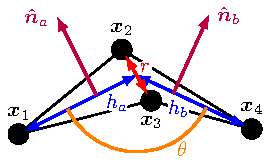
\includegraphics{BAHschematic.pdf}
  \caption{\label{fig:ell-BAHschematic}
    Schematic of the bar and hinge model showing the relevant parameters for a single hinge element.
    $h_i$ and $\bm{\hat{n}}_i$ denote the height and unit normal of each triangle respectively.
  }
\end{figure}

The expressions for the gradient of the energy can be obtained by considering the stretching and bending energies of an individual bond and hinge.
For simplicity, the indices for the bond and hinge are ignored.
Using the variables shown in the schematic in \cref{fig:ell-BAHschematic}, the gradient of the stretching energy of the bond between $\bm{x}_2$ and $\bm{x}_3$ is given by
\begin{equation}
  \frac{\partial E^\text{S}}{\partial \bm{x}_2} = - \frac{\partial E^\text{S}}{\partial \bm{x}_3} = k^\text{S} (r - r_0) (\bm{x_2} - \bm{x_3}).
\end{equation}
The gradients of the bending energy of the hinge are
\begin{align}
  \frac{\partial E^\text{B}}{\partial \bm{x}_1} &= k^\text{B} (\theta - \theta_0) \frac{\bm{\hat{n}}_a}{h_a}, \\
  \frac{\partial E^\text{B}}{\partial \bm{x}_2} &= - k^\text{B} (\theta - \theta_0) \left[\frac{\bm{\hat{n}}_a}{h_a} + \frac{\bm{\hat{n}}_a + \bm{\hat{n}}_b}{r}\right],
\end{align}
\begin{align}
  \frac{\partial E^\text{B}}{\partial \bm{x}_3} &= - k^\text{B} (\theta - \theta_0) \left[\frac{\bm{\hat{n}}_b}{h_b} + \frac{\bm{\hat{n}}_a + \bm{\hat{n}}_b}{r}\right], \\
  \frac{\partial E^\text{B}}{\partial \bm{x}_4} &= k^\text{B} (\theta - \theta_0) \frac{\bm{\hat{n}}_b}{h_b}.
\end{align}

These models have been widely applied to study origami structures \cite{Liu2017a,Gillman2018,Zhou2023}, where the triangular mesh is made to match the geometry of the crease pattern.
Alternatively, it can also be used to model continuous elastic surfaces by choosing the spring constants in such a way that they accurately represent the elastic moduli in the continuum limit.
In which case, the spring coefficients are given by \cite{Gelder1998,Seung1988,Grinspun2006},
\begin{gather}
  k_\text{S} = Yt \cdot \frac{A_\text{sum}}{r_0^2}, \\
  k_\text{B} = \frac{Yt^3}{12(1-\nu^2)} \cdot \frac{r_0^2}{A_\text{sum}},
\end{gather}
where $Y$ is the Young's modulus, $t$ is the thickness of the surface, and $\nu$ is the Poisson's ratio.
The value $A_\text{sum}$ is the total area of the adjacent triangles at equilibrium, of which there will be one for bonds on the boundary, and two for the others.
This method is used if the rigidities have not been directly set, and the \code{thickness} parameter is provided.
This can take a different value for each node of the mesh in order to create a varying thickness.
In this case an average is taken for each bond and hinge.

This model is particularly useful for its simplicity and speed, however it has some limitations on its accuracy compared to real structures.
Firstly, because it is a 2D surface, the thickness is assumed to be much smaller than the dimensions along the surface itself.
This is particularly important since the one-dimensional folding of adjacent triangles cannot accurately model the effect of twisting, but this will be negligible as long as the thickness is sufficiently small.
This is because any twisting of a thin surface requires some in-plane stretching, the energy of which scales proportionally to the thickness, $t$, while twisting energy scales as $t^3$.
Similarly, it cannot model the energy due to Gaussian curvature, the product of the two principal curvatures.
However, the high resistance to stretching makes this negligible in most circumstances, and, if the boundary is fixed or the surface is closed, the total energy due to the Gaussian curvature is topologically constant according to the Gauss-Bonnet theorem \cite{Rueda-Contreras2021}, so it may be safely ignored.
Finally, another limitation of the model is that the Poisson ratio under stretching cannot freely be tuned.
Instead, it depends upon the geometry of the mesh.
For example, if an equilateral triangular mesh is used then the Poisson ratio will be 1/3, regardless of the spring constants that are applied \cite{Gelder1998}.
These limitations mean that the model is primarily of use to study elasticity problems where bending is the dominant effect.

An additional energy contribution is possible by incorporating an external force with the \code{force} parameter.
This can be a uniform force to model gravity, or a magnetic field; or applied inhomogeneously across the structure such as to initialise random structures.
It is also possible to include interactions with a substrate using \code{setWall}, which turns on a Lennard-Jones 3-9 potential, which is obtained by considering an interaction between a particle and an infinite wall of particles that interact by the standard Lennard-Jones potential, \cref{eq:ell-lj}.
\begin{equation}
  E(h) = \epsilon \left( \frac{2}{15}\left(\frac{\sigma}{h-h_0}\right)^9 - \left(\frac{\sigma}{h-h_0}\right)^3 \right),
\end{equation}
where the height above the wall, $h$, has been shifted by $h_0$ to ensure that the energy is minimal at $h=0$.
The Lennard-Jones parameters $\sigma$ and $\epsilon$ are initially set to $10^{-12}$ and $10^{-5}$, which tend to give results that correspond to levels of adhesion observed in experiments.
But the precise adhesion energy, controlled by $\epsilon$, will depend upon system size and so should be adjusted for different applications.
The adhesion arises because the potential is attractive for $h>0$, but if this is not desired, it can be switched of, in which case the potential is cut off at $h=0$ and shifted so that $E(0)=0$.

This potential uses the software's parallel framework by splitting the contributions to the energy into energy elements.
The stretching energy uses one element for each pair of particles, and the bending energy has one element for the four particles in pair of triangles.
If the force and substrate interactions are switched on, they each have one element per particle.


\subsection{Phase Field Model}
In order to model multicomponent fluid systems a phase field model has been implemented, \code{PFWetting}.
This potential has been implemented with two variants: a binary fluid and an $N$-fluid version, which can be accessed by modifying the \code{nFluid} parameter.
This method uses a square grid (resolution size $\delta$) where each node is marked as either solid or a fluid using \code{setSolid}.
If a fluid node is adjacent to a solid node then the solid surface passes through the center of the node, and the volume $V$ and surface area $A$ take different values from the bulk.
Each fluid has a concentration, $C_i$, for each fluid $i$ (for the $N$-fluid variant) or an order parameter, $\phi = C_1 - C_2$ for the binary model.
These concentrations take bulk values of 0 or 1 depending on if the fluid is located at that position, and smoothly vary, resulting in diffuse fluid interfaces.

This potential has four or five contributions to the overall energy depending upon whether it is using the binary or $N$-fluid model.
One sets the bulk fluid values, $E^\text{B}$, and another includes the interfacial energy of the fluids, $E^\text{I}$.
If the $N$-fluid model is used, there is also a soft energy constraint to ensure that the total concentration is the same everywhere, $E^\text{D}$.
Next, there is a fluid-solid interaction, $E^\text{S}$.
Then, finally, there is either an energy penalty to set a constant volume across the system, $E^\text{V}$, or the energy due to the pressure of the system, $E^\text{P}$.

The $E^\text{B}$, $E^\text{I}$, and $E^\text{D}$ terms each apply to the whole of the fluid domain.
Therefore, they are split into single elements for each fluid node in the system so that the potential can be computed in parallel.
The energies of these discrete elements are then given by,
\begin{equation}
  E^\text{B} =
  \begin{cases}
    \frac{\kappa}{16} (\phi + 1)^2 (\phi - 1)^2 V & \text{binary},\\
    \sum_{i=1}^{N} \frac{\kappa_i}{2} C_i^2 (C_i - 1)^2 V & \text{$N$-fluid},
  \end{cases}
  \label{eq:ell-PFEB}
\end{equation}
\begin{equation}
  E^\text{I} =
  \begin{cases}
    \frac{\kappa'}{4} (\grad \phi)^2 V & \text{binary},\\
    \sum_{i=1}^{N} \frac{\kappa'_i}{2} (\grad C_i)^2 V & \text{$N$-fluid},
  \end{cases}
  \label{eq:ell-PFEI}
\end{equation}
\begin{equation}
  E^\text{D} =
  \begin{cases}
    0 & \text{binary},\\
    k^\text{V} \left( 1 - \sum_{i=1}^{N} C_i \right)^2 V & \text{$N$-fluid}.
  \end{cases}
  \label{eq:ell-PFED}
\end{equation}
\Cref{eq:ell-PFEB} uses a double well potential to ensure that the energy is minimised when the fluid concentrations are 0 or 1.
\Cref{eq:ell-PFEI} penalises any fluid interfaces where the gradient of the concentrations / order parameters are non-zero.
\Cref{eq:ell-PFED} ensures that the sum of the concentrations is equal to one by using a large constraint coefficient $k^\text{V}$.
The parameters $\kappa_i$ and $\kappa'_i$ are related to the interfacial tensions, $\gamma_{ij}$, and widths, $\alpha_{ij}$.
This can be determined by finding the fluid concentration function that minimises the energy given by the continuous analogue of \cref{eq:ell-PFEB,eq:ell-PFEI}, giving the following relations,
\begin{gather}
  \gamma_{ij} = \frac{\sqrt{\kappa_i+\kappa_j} \sqrt{\kappa'_i+\kappa'_j}}{6},\\
  \alpha_{ij} = \sqrt{\frac{\kappa'_i+\kappa'_j}{\kappa_i+\kappa_j}}.
\end{gather}
They are assigned by the \code{setSurfaceTension} and \code{set\-Interface\-Width} functions, and used to calculate $\kappa_i$ and $\kappa'_i$.
However, if four or more fluids are used, the full set of surface tensions cannot be matched because there are not enough parameters in the model.
Alternative models that allow all surface tensions to be prescribed are available in the literature, such as \cite{Dong2018}.

Each of these energy elements includes the neighbouring nodes in order to calculate the gradients in \cref{eq:ell-PFEI}.
Generally these use central difference, however forward difference is used if one side is a solid node.
For example, the $x$-gradient of $\phi$ at a point where $x=x_0$ is
\begin{equation}
  \frac{\partial \phi}{\partial x} =
  \begin{cases}
    \frac{\phi(x_0+\delta) - \phi(x_0-\delta)} {2\delta} & \text{for bulk fluid},\\
    \frac{\phi(x_0+\delta) - \phi(x_0)} {\delta}         & \text{if solid at $x_0-\delta$},\\
    \frac{\phi(x_0) - \phi(x_0-\delta)} {\delta}         & \text{if solid at $x_0+\delta$}.\\
  \end{cases}
\end{equation}
The equations for the energy gradients at each element are therefore given by
\begin{align}
  \frac{\partial E^\text{B}}{\partial \phi} = \frac{\kappa}{4} \phi (\phi^2 - 1) V \qquad& \text{binary},\\
  \frac{\partial E^\text{B}}{\partial C_i} = \sum_{i=1}^{N} \frac{\kappa_i}{2} (2C_i^3 - 3C_i^2 + C_i) V \qquad& \text{$N$-fluid}.
\end{align}

The interaction between the fluid and solid is designed to apply partial wetting behaviour, such that the fluid interface meets the solid surface at a specific contact angle, $\theta$.
This contact angle can be defined by a function across the domain using \code{setContactAngle}.
The interaction uses a cubic wetting potential, where the gradient is zero at the bulk fluid concentrations in order to avoid enrichment of the fluid concentration at the surface.
This energy relies only upon the local fluid values at the surface, so the energy is split into one element per surface node with
\begin{equation}
  E^\text{S} = \frac{1}{\sqrt{2}} \cos{\theta} \left( \frac{\phi^3}{3} - \phi - \frac{2}{3} \right) A.
\end{equation}

Finally the pressure and volume energies are given by,
\begin{gather}
  E^\text{P} = p V_\text{tot},\\
  E^\text{V} = k_\text{V} (V_\text{tot} - V_0)^2,
\end{gather}
where $p$ and $V_0$ are the chosen pressure and volume, and $V_\text{tot}$ is the total volume of the fluid.
Unlike the energy contributions, the calculation of $V_\text{tot}$ relies upon the whole system, so it cannot be assigned to separate energy elements and requires special treatment using the \code{blockEnergyGradient} function.
Therefore, the fluid volume is first calculated on each block and then added up across the processors, reducing the overhead required for MPI.



\section{Implementation of minimisation methods}
The \code{Minimiser} class contains the framework for optimising a single state to a (usually local) minimum in the energy landscape.
Therefore, it does not encompass ensemble minimisation methods, such as Genetic Algorithm, which will be discussed in the next section.
The methods that have been implemented are:
\begin{itemize}
  \item Gradient descent (\code{GradDescent})
  \item L-BFGS (\code{Lbfgs})
  \item FIRE (\code{Fire})
  \item Simulated annealing (\code{Anneal})
\end{itemize}


These methods are themselves subclasses of \code{Minimiser} and implement functions that are called during a minimisation.
The first is an \code{init} function that can be used if any set up is required at the start, including the instantiation of parameters.
Then the main loop is run, during which the \code{iteration} function is called which contains the main part of the methods.
At the end of each iteration a \code{checkConvergence} function detects if it has reached the minimum, at which point the method ends.
A user defined function may also be passed into the minimisation that is called at the start of each iteration to modify system parameters.
This provides flexibility to the user and could be used, for instance, to steadily perturb the system during the start of the minimisation, or to save the trajectory of the minimisation.

\code{Minimiser} also has parameters generic to most or all of its subclasses.
Namely, the maximum number of iterations and which line search method should be used, if at all.
Currently, backtracking line search is included, which ensures that the energy decreases sufficiently to satisfy the Armijo rule, \cref{eq:lm-ls-armijo}, with $c_1=0.5$, or optionally, that the energy never increases more than a chosen amount.

\subsection{Gradient descent}
The gradient descent implementation has one additional parameter \code{alpha}, which is the step size factor, $\alpha_i$, in \cref{eq:lm-graddescent}.
This has a default value of $0.1$, although the actual step size will be determined using a line search.
So, unless it is turned off, the value of \code{alpha} is not hugely important.
In order to check for convergence, the root mean square of the gradient, $\abs{\grad E} / \sqrt{N}$, where $N$ is the number of degrees of freedom, is compared to the \code{convergence} parameter that is chosen for the \code{State} object.
This same criterion is also used for both L-BFGS and FIRE.

The gradient descent algorithm is also very amenable to parallelisation by distributing the degrees of freedom between processors.
This is because communication between the processors are only required at three points: to communicate the gradient to the halo nodes, computing the magnitude of the gradient for the root mean square, and calculating the energy for the line search.
The latter may require multiple communications, depending upon the number of iterations, but if no line search is used then just the two communications are necessary.

\subsection{L-BFGS}
As for the implementation of L-BFGS, there are two additional parameters.
The first is the number of steps to store to calculate the search direction, $m$, which has a default value of five.
Secondly, \code{maxStep} can be used to restrict the step size in each iteration, such that, if the step is greater than this, it is rescaled to the maximum value.
This can be useful, for example, to ensure that the minimisation is smooth when the trajectory is used to approximate an MEP.
If this value is not manually set, then no restriction is made.

Currently, if L-BFGS is run in parallel, then only the calculations of the gradient and line search are split among the processors, while the calculation of the search direction is instead performed in serial.
This is because $2m+2$ dot products are required when calculating \cref{eq:lm-lbfgs-q0,eq:lm-lbfgs-q,eq:lm-lbfgs-z0,eq:lm-lbfgs-z}, and each would require a separate communication.
Therefore, the search direction is calculated in serial by collecting the whole of the gradient on each processor in an attempt to reduce the number of MPI communications.

\subsection{FIRE}
The \code{Fire} object has a parameter \code{dtMax}, which is the maximum timestep that is allowed when updating the velocity and the position.
Ideally, an appropriate value should be assigned by the user.
However, if none are provided, then a reasonable value will be estimated using the energy gradient at the start of the initialisation,
\begin{equation}
  \Delta t_\text{max} = \frac{1}{10 \sqrt{\abs{\grad E}}}.
\end{equation}
This will result in a step size that is independent of the scale of the energy, so, if the gradients are very high it will not cause very large step sizes.
The step size would instead be on the order of $0.1$, which may not be accurate for particularly large or small system sizes.
In the unusual circumstance that the gradient is initially zero, \code{dtMax} is simply set to one.
Since FIRE is an inertial optimisation method that uses a continually updated velocity, the line search is off by default.
However, it can be switched on, in which case the importance of the timestep is reduced.

In contrast to L-BFGS, FIRE does not require so many communications between processor nodes, and so is efficient for parallelisation.
Aside from communicating to update the halo nodes, the only other communication that is required is to calculate the magnitudes of the gradient and the velocity, and their dot product.
Therefore the method never requires collecting all degrees of freedom on a single processor.

\subsection{Simulated Annealing}
To use simulated annealing an \code{Anneal} object can be created using two parameters: \code{displacement} and \code{tempInit}.
Suitable values for these cannot be easily guessed, so the user is required to provide them.
The former is used in calculating the random trial state for each iteration.
For each degree of freedom a perturbation is picked from a uniform distribution where the maximum value is given by \code{displacement}.
The second parameter \code{tempInit} describes the initial temperature, which should be high enough to allow the system to adequately explore the energy landscape.
The precise function describing how the temperature decreases over time may be set by the user using the \code{coolingSchedule} parameter, but the default function uses linear multiplicative cooling \cite{Junn2017}, such that, at iteration $i$, the temperature is
\begin{equation}
  T(i) = \frac{T_0}{1 + ki},
\end{equation}
where $T_0$ is the initial temperature, and $k$ is the cooling rate, which can be adjusted via the parameter \code{coolingRate} which has a default value of 1.

Because simulated annealing is not a gradient-based minimiser and it is attempting to find the global minimum rather than local minima, convergence should not be determined using the root mean square of the gradient.
Instead, the state is determined to be converged once the trial state has been rejected more than a certain number of iterations in a row, which is given by the \code{maxRejections} parameter.
This is initially set to zero, in which case the method is allowed to continue until it reaches the maximum number of iterations.

Simulated annealing is performed almost completely in parallel.
The only communications required are to sum up the total energy of the state, to communicate the random perturbations to the halo coordinates, and to share the same random test value so that all processors agree on whether to accept or reject the step.



\section{Implementation of energy landscape methods}
The main ELLib library contains the more general energy landscape methods that typically make use of the minimisation algorithms in order to find transition states, pathways, and in the search for minima.
Because they cover a variety of methods, they do not follow any rigid structure, unlike the minimisation methods.
Each method is implemented in a class which can be used by creating an object for the method, modifying any parameters, and then calling a \code{run} function.
This function outputs the result for the method, whether that be a global minimum configuration, transition state, or pathway.
Each class may also have functions for obtaining other information from the method.

The currently implemented methods are the genetic algorithm for finding global minima, the BITSS method for locating transition states, and NEB to find pathways.
In the future we hope to expand this to include other methods, such as basin hopping, eigenvector-following, and the string method.


\subsection{Genetic Algorithm}
The genetic algorithm is implemented in the \code{GenAlg} class.
This takes a \code{Potential} object that is be used to generate a population of states.
The size of this population is given by \code{popSize}, and the total number of generations, \code{maxIter}.
Each of these are initially set to 100.

There are two possibilities for initialising the population.
Firstly, a function may be provided by the user to individually generate states (assiged using \code{stateGen}).
Alternatively, \code{bounds} can be set to the upper and lower bounds for each degree of freedom.
The coordinates for the states are then randomly generated between these bounds.
If neither of these are set then there is no way of determining suitable coordinates for the states, so the method will not run.

In order to create a new generation, the parents can be selected using one of two methods, either roulette selection (the default), or simply choosing the most fit.
This is set by the \code{selectionMethod} parameter, with the number of parents chosen as fraction of the population according to \code{selectionRate}.
Elitist selection is also possible by setting \code{numElites} to be the number of the best states that should be passed directly to the next generation.
The remaining children are then created using uniform crossover between pairs of parents.
Each of the child's coordinates may then be mutated with a probability given by \code{mutationRate}.
This mutation is chosen from a uniform distribution with a standard deviation chosen by the \code{perturbation} parameter.
If this is not set, but the bounds are, then the standard deviation is 1\% of the total allowed range.

The genetic algorithm implementation also has a couple of other useful features.
Firstly, it can also be run as a Lamarckian hybrid approach by passing a \code{Minimiser} object to use for the local search.
This allows it to more quickly identify and explore local minima in the landscape.
Secondly, a generic user-defined function can be called in each generation to access and modify the population.
This can be used, for example, to output the fittest state from each generation.

The standard behaviour is to continue until the full number of generations has been reached, but there are two possible methods for stopping early if it is deemed to have converged.
The first is a user-defined energy limit, such that if a state is found with a lower energy it will stop.
This could be useful if the precise global minimum is not needed and all that is desired is a low energy solution.
The second method halts the method if it has gone a certain number of generations without seeing any improvement in the fittest individual.
These two methods and their criteria can be applied using the \code{setConvergence} function.

The method by which the genetic algorithm is parallelised depends on the number of processors relative to the size of the population.
If the population size is greater than or equal to the number of processors then each state is run on just a single processor.
This is particularly efficient because the processors only need to communicate when setting each new generation, while the energy of each state is computed in serial.
On the other hand, if there are more processors, then each state is distributed among two or more processors.
This may be useful if the potential is particularly complex or a hybrid method is being used.
This parallelisation is most efficient when the population size is a multiple / factor of the number of processors.
Otherwise, some processors will be assigned a larger share of the work, and the others will spend time idle.

\subsection{BITSS}
The \code{Bitss} class provides the implementation of the BITSS method, and is initialised using two states and a minimiser.
These two states provide the initial coordinates for the method, so they are typically selected to be the minima.
The \code{Bitss} class creates a new \code{State} object and an associated \code{BitssPotential}.
These wrap around the two individual states in order to calculate the full energy of the pair of states, including the constraints.

The most significant parameter for BITSS is the fraction to reduce the distance for each iteration.
This is given by \code{distStep} with a value of 0.5, but this may be too rapid for some applications, and should be changed accordingly.
Typically, the method should run until convergence or failure, but \code{maxIter} can be set to halt the method after a large number of iterations, with an initial value of 100.
If \code{distStep} is reduced significantly then this will likely need to be increased.
To calculate the separation between the states the Euclidean distance is often used, but the user is free to use any metric.
This can be done by passing functions for the distance and its gradient to the \code{distFunc} parameter.

The constraint coefficients are recalculated throughout each minimisation according to the \code{coefIter} parameter, which is initially every 100 iterations.
During this recalculation the energy barrier is estimated using a linear interpolation, but for some applications this may be many orders of magnitude too large when the states are far from TS.
To prevent this from causing an issue, the \code{maxBarrier} parameter may be set to a reasonable value.
It is also possible to alter the $\alpha$ and $\beta$ parameters from \cref{eq:bitss-ke,eq:bitss-kd}, using \code{alpha} and \code{beta}, but they can usually be left at their recommended values of 10 and 0.1, respectively.
To prevent issues associated with recalculating the coefficients, it is recommended to switch off the line search for the minimisation.
Furthermore, if no minimiser is provided then it defaults to L-BFGS with the line search automatically switched off.

The convergence to the TS can be based on one of five methods.
Two of these are based upon the separation constraint reaching a chosen size, whether that be the actual distance, or the distance relative to the initial separation.
The next criteria are based upon the estimate of the TS.
The third criterion relates to the root mean square of the gradient at the estimate, while the fourth uses the change of the estimate from one iteration to the next.
Finally, the uncertainty of the TS energy can be used.
This is calculated as the difference between the energy of the TS estimate, $E_\text{TS}$, and the pair of states, $E_i$, relative to its height above the initial state energies, $E_{i,0}$,
\begin{equation}
  \epsilon_E = \frac {E_\text{TS} - \langle E_1, E_2 \rangle} {E_\text{TS} - \langle E_{1,0}, E_{2,0} \rangle},
\end{equation}
where $\langle\cdots\rangle$ denotes the average.
Each of these methods can be set using the \code{set\-Convergence\-Method} function, which is initially set to a relative distance criteria of 1\%.

The coordinates of the TS are output by the \code{run}, but other information can also be extracted.
The final two states can be obtained using the \code{getPair} and \code{getPairCoords} functions, which return two \code{State} objects or vectors, respectively.
Meanwhile, the \code{getTS} and \code{getTSCoords} functions give the state and coordinates of the TS estimate midway between the pair.
\code{Bitss} can also report if it believes it has not successfully found the TS if the \code{getFailed} function is called.
This is based upon any of three conditions: if the final state did not properly converge, if $\langle E_1, E_2 \rangle < \max(E_{1,0}, E_{2,0})$, or if $E_\text{TS} < \langle E_1, E_2 \rangle$.

The BITSS method can be run in parallel to distribute the calculation of the energies and gradients of the individual states, but the energy contributions of the constraints are computed in serial.
This is because the total energy needs to be known for the energy constraint, and the full set of coordinates are needed to calculate the separation between the two states.
However, the effect of this is relatively minor because the calculation of the underlying potential tends to be much more costly.

% \subsection{Climbing Image}

\subsection{Nudged elastic band (NEB)}
The \code{Neb} class encompasses several variations of the NEB method, including a hybrid climbing image method and DNEB.
The latter of which may also be accessed using the \code{Dneb} wrapper class.
There are two ways that the method may be initialised, either using a set of coordinates for the initial chain, or by passing the end points and the number of states (including the end points), in which case the chain is set by a linear interpolation.

Similar to BITSS, the NEB implementation uses a single \code{State} object with \code{NebPotential} which calculates the total energy of the elastic band.
This delegates the computation of the single state energies to a set of \code{State} objects for each image along the chain.
This main \code{State} is then minimised to find the pathway.
Because NEB and DNEB modify the gradient of the energy, the minimisation should, again, not use a line search, and the default L-BFGS minimiser has it switched off by default.

The elastic spring constant, $k$ in \cref{eq:lm-neb-energy}, can be set using the \code{kSpring} parameter, which is initially set to one.
This should not be too large or too small because it may cause the potential or equal spacing constraint to be washed out and the method may take longer to converge.
The tangent vectors used to project the components of the forces are obtained using the bisection method, described by \cref{eq:lm-neb-taubisect}.

To utilise a hybrid climbing image method the \code{setHybrid} function may be called.
This is also used to set the \code{hybridIter} variable, which activates the climbing image at a chosen iteration, allowing the the chain to first approximate the pathway.
After this, at each iteration, the state with the highest energy is selected and its driving force is replaced by the climbing image force, \cref{eq:lm-ci-force}.

The \code{run} function performs the initialisation and optimisation of the chain and outputs the coordinates along the pathway.
Subsequent outputs can be acquired using \code{getChain}, \code{getCoords}, and \code{getEnergies}.
These methods provide the final list of \code{State} objects, the list of coordinates, and the list of energies, respectively.

The method allows the chain of states to be distributed among the available processors so that the calculations of the single state energies and gradient are performed in parallel.
These are either allocated with multiple states per processor or multiple processors per state, using the same approach as the genetic algorithm.
The results from the individual states are then broadcast to all processors so that the total energy and gradient can be computed serially.
Although the full energy and gradient could possibly be calculated in parallel, this would significantly complicate the method, and much like BITSS, the main computational cost is usually associated with the single state energy calculations.

% \subsection{Benchmarking}
% \subsubsection{Minimisation}
% \subsubsection{Transition state search}

% \subsection{Parallelisation}
% In order to study how the methods scale under parallelisation, 2D wetting simulations are performed using the \code{PFWetting} potential and their runtimes are recorded.
% A $90\times90$ system size is used for this with a solid surface at the bottom, which has alternating hydrophilic and hydrophobic regions with contact angles of $60^\circ$ and $120^\circ$, respectively.
% The total volume of the liquid is constrained to that of a semi-circular drop with radius of 30 in lattice units, which is used to initialise the minimisation tests.
% The various system parameters are: \code{interfaceSize}$=1$, \code{surfaceTension}$=1$, \code{volConst}$=10^4$, and a root-mean-square gradient convergence criteria of $10^{-4}$.
% The minima and transition state for this system are shown in \cref{fig:ell-parallel}(a).

% \begin{figure}[htb]
%   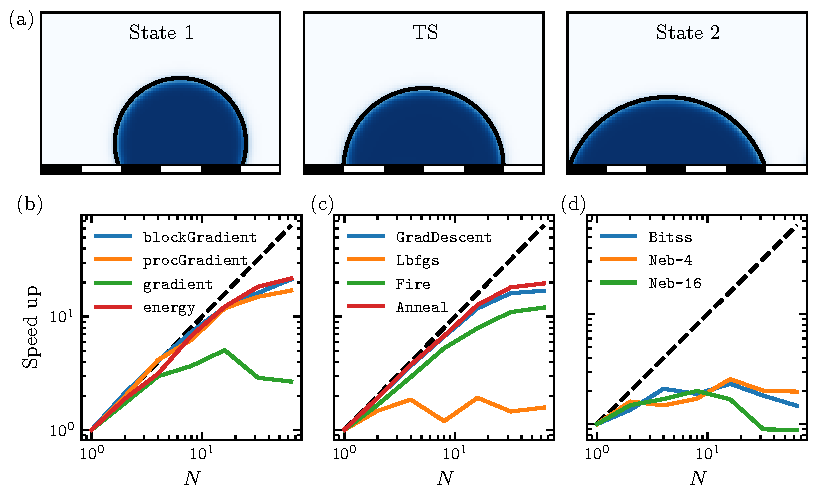
\includegraphics{parallel.pdf}
%   \caption{\label{fig:ell-parallel}
%     (a) The stable states and transition state for the parallelisation test system.
%         The top third of the simulation height has been removed.
%         Black regions indicate hydrophilic sections of the solid, and the white regions are hydrophobic.
%     (b-d) Comparison showing how much the runtime is reduced with different numbers of processors, $N$, compared to a single processor for each method.
%           The dashed line shows the optimal speed up (equal to the number of processors).
%     (b) Energy and gradient calculation methods.
%     (c) Minimisation methods.
%     (d) Energy landscape methods.
%   }
% \end{figure}

% First, various energy and gradient functions are tested by randomly altering the local coordinates and then computing the function \num{100000} times.
% These each perform different types of MPI communication, so it is a useful indication of how significant each becomes as the number of processors are increased.
% Specifically, \code{energy} sums a single value across the processors, \code{gradient} collects all of the degrees of freedom onto a single processor, \code{procGradient} communicates the halo regions, and \code{blockGradient} performs no communication at all.
% The results, in \cref{fig:ell-parallel}(b), show a similar trend for all of the functions with the exception of \code{gradient}.
% These are not far from the ideal scaling behaviour, showing that they are well parallelised.
% Indeed, the drop-off at 32 and 64 processors also occurs in \code{blockGradient} even though there is no MPI communication.
% So, it must be primarily due to increased computation from the size of the halos becoming equivalent or larger than the main blocks, so a larger system size will give even more efficient scaling behaviour.
% On the other hand, the poor behaviour of \code{gradient} shows that gathering all of the degrees of freedom onto a single processor requires much more computational overhead, and leads to worse performance beyond a certain number of processors.
% Therefore, methods that rely upon \code{gradient} or otherwise gather all degrees of freedom will likely also see poor scaling behaviour.

% Next the minimisation methods are tested by initialising a semi-circular droplet in the middle of the solid and allowing it to converge.
% L-BFGS is by the far the fastest at this, converging in \num{7943} iterations, or about five and a half seconds using a single processor.
% Meanwhile, FIRE takes \num{749557} iterations (over 400 seconds) to converge to the same degree, while gradient descent and simulated annealing are still far from convergence after \num{1000000} iterations, at which point they are stopped.

% However, the results for the performance under an increasing number of processors, \cref{fig:ell-parallel}(c), are that opposite.
% Here, the slowest methods, gradient descent and simulated annealing, see the best scaling behaviour, with FIRE not far behind.
% This is because these methods only rely upon the \code{procGradient} function which scales efficiently, and their whole methods are parallelised.
% Whereas, L-BFGS only sees a moderate increase in speed because it uses the more costly \code{gradient} function and does not distribute the calculation of the step during each iteration.
% So, even though it is the fastest method, it will not be able to significantly benefit from parallelisation to simulate large-scale systems.

% By timing the sections of the L-BFGS algorithm we find that only about 70\% of the time is spent computating the potential when using a single processor.
% So under the current implementation it could only speed up by a maximum of about three times, even before considering the effect of MPI communication.
% Therefore, L-BFGS would considerably benefit from a true parallel implementation, such as described by Fei et al.\cite{Fei2014}.

% Next, the energy landscape methods are investigated.
% Namely, BITSS and NEB with 4 and 16 images along the chain.
% These are initialised using the two states shown in \cref{fig:ell-parallel}(a).
% BITSS is able to converge to the transition state in under 130 seconds on a single processor.
% However, NEB struggles for this system (as discussed in \cref{ch:bitss}), so it is simply run for \num{10000} iterations, which takes about 160 seconds for 4 images and \num{1200} seconds for 16 images.
% \Cref{fig:ell-parallel}(d) shows the results, in which, unfortunately neither method sees a significant increase in speed.
% This is because they each use L-BFGS for the minimisation, and, similarly, collect the full set of coordinates and perform a serial computation.

% Overall, future work should look at implementing a full parallel version of L-BFGS and the energy landscape methods, or identifying alternative methods that scale more efficiently.


\section{Demonstration: structural optimisation}\label{sec:ell-demo}
In this section the versatility of the software library will be demonstrated by optimising an elastic structure to maximise the energy barrier between two states, thereby identifying the structure for which these states are at their most stable.
The structure that will be investigated is a table-shaped buckled mesostructure that will be studied in further detail in the next chapter.
\Cref{fig:ell-structopt}(a) shows a schematic of this structure with the four parameters that will be optimised: the leg width, the thickness, and the outer and inner radii of the centre.
At the end of legs are bonding sites that are compressed by a 20\% strain and then fixed in place.
The structure will not restricted by a substrate, so may buckle down as well as up.
The two stable states, between which the barrier will be computed, are shown in \cref{fig:ell-structopt}(b).

The parameters are bounded during the optimisation to ensure that they remain realistic.
The thickness, for example, would likely continue to rise if left unrestricted.
Therefore, a maximum is placed to ensure that it does not become unreasonably large and respects the model's requirement that the thickness remains relatively small compared to the other dimensions of the structure.
The parameters are given relative to the total length of the structure, ignoring binding sites, which is given a size of 1.
It also depends upon the resolution of the mesh, which is made as close as possible to an equilateral triangular mesh with side lengths of 0.05.
These parameter bounds are listed in \cref{tab:ell-structbounds}.
The other fixed parameters are listed in \cref{tab:ell-params}.

\begin{table}[htb]
  \begin{tabularx}{0.5\textwidth}{ccc}
    \hline\hline
    Parameter      & Minimum & Maximum \\
    \hline
    $w$            & 0.0866$^a$ & 0.25 \\
    $t$            & 0       & 0.05 \\
    $r_\text{out}$ & 0       & 1/3 \\
    $r_\text{in}$  & 0       & $r_\text{out}$ \\
    \hline\hline
  \end{tabularx}
  \footnotesize{\\$^a$ This is two times the optimal triangular height.}
  \caption{\label{tab:ell-structbounds}
    The bounds on each of the four structural parameters.
  }
\end{table}

To perform this structural optimisation it is necessary to combine a variety of energy landscape methods.
First, energy minimisation is required to identify the two stable states for each set of parameters.
L-BFGS will be used for this.
Then, the transition state between the states will be identified using BITSS.
At this point the energies of the TS, $E_\text{TS}$, and minima, $E_{1/2}$, are known, so the energy barriers in each direction can be evaluated and added together to give the `total energy barrier',
\begin{equation}
  E_\text{B} = 2E_\text{TS} - E_1 - E_2.
  \label{eq:ell-totbarrier}
\end{equation}
To maximise this, the four structural parameters will be optimised using the genetic algorithm.
A script is written that carries out this procedure using ELLib, with its structure described here.

In order to be used with the genetic algorithm a \code{Potential} subclass is created, whose energy is the inverse of the barrier given in \cref{eq:ell-totbarrier}.
Therefore, minimising this energy will maximise the barrier.
The potential also takes a blank function for the gradient because the genetic algorithm does not require it.

The energy function takes four coordinates between 0 and 1, which it converts into the parameters using the bounds in \cref{tab:ell-structbounds}.
An external program is then called to generate a mesh based upon the parameters, using a Delaunay triangulation \cite{Rebay1993} to make the triangles as close to equilateral as possible.
Using this mesh, the thickness, and the \code{BarAndHinge} potential, an initial \code{State} object is created.
Two copies of this state are then minimised using \code{Lbfgs}, each with a function that is called for the first 500 iterations of the minimisation.
This function has two roles.
First, it slowly moves the binding sites in until they reach the final position.
Second, it applies forces to the structure to obtain the desired configuration.
After 500 iterations these are turned off to allow the structure to relax.
Once the states have converged, they are checked to ensure they converged correctly.
If not, the energy barrier is determined to be zero, and the function ends.
Otherwise, the two minimum states are passed to \code{Bitss} in order to find the TS.
At this point the barrier is evaluated using \cref{eq:ell-totbarrier}, and the function returning the inverse of this value.

Using this potential, the script creates a \code{GenAlg} object and sets the following parameters: $\code{popSize}=48$, $\code{maxIter}=20$, $\code{bounds}=[0,1]$, $\code{perturbation}=0.3$, $\code{mutationRate}=0.25$, $\code{selectionRate}=0.4$.
Additionally, it uses elitism to ensure the best structure is not lost, and it uses a function to save the population in each generation.
Finally, the genetic algorithm is run until the full 20 generations are complete.

\begin{figure}[htb]
  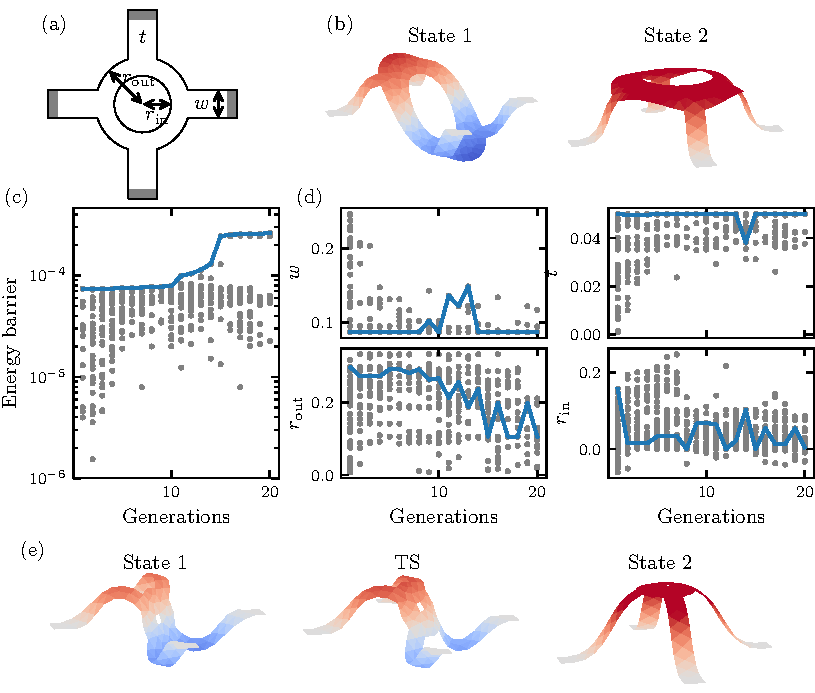
\includegraphics{structopt.pdf}
  \caption{\label{fig:ell-structopt}
    (a) Schematic of the structure showing the four parameters: leg width, $w$, thickness, $t$, outer radius, $r_\text{out}$, and inner radius, $r_\text{in}$.
        The fixed bonding sites are shown in grey.
    (b) The two minima for the structure with the highest barrier in the first generation.
        The colour represents the height above the horizontal plane, positive height in red, negative in blue.
    (c) The energy barrier for each individual in the population.
        The blue line follows the states with the highest barrier in each generation.
    (d) The values for each of the four parameters for each individual throughout the optimisation process.
        The parameters are scaled such that the total length of the structure, excluding bonding sites, is 1.
    (e) The minima and transition state for the most optimal state after 20 generations.
  }
\end{figure}

The results in \cref{fig:ell-structopt} show how the optimal structure evolves over time.
The leg width and thickness very quickly converge to their lower and upper bounds, respectively, and the inner radius also becomes small early on.
However, the outer radius takes more time to evolve, beginning with a large value, and only changing to a small radius around generation 15, at which point the maximum barrier correspondingly increases.
After 20 generations the optimal structure is: $w=0.0866$, $t=0.05$, $r_\text{out}=0.1145$, and $r_\text{in}=0.0137$.

These results demonstrate that a highly complex optimisation study is feasible using ELLib, and more generally, illustrates the flexibility of the library.

\begin{table}[]
  \begin{tabularx}{\textwidth}{>{\hsize=.5\hsize\linewidth=\hsize}C >{\hsize=.75\hsize\linewidth=\hsize}C >{\hsize=2\hsize\linewidth=\hsize}C >{\hsize=.75\hsize\linewidth=\hsize}C}
    \hline\hline
    Topic & Symbol & Parameter description & Value \\
    \hline
    \multirow{5}{*}{\rotatebox[origin=c]{90}{Structure}}
          & ---   & Compressive strain     & 20\% \\
          & ---   & Total structure length & 1 \\
          & ---   & Mesh resolution        & 0.05 \\
          & $Y$   & Young's modulus        & 1.4 \\
          & $\nu$ & Poisson ratio          & 0.3 \\
    \hline
    \multirow{5}{*}{\rotatebox[origin=c]{90}{BITSS}}
          & $\alpha$ & Energy constraint strength         & 10 \\
          & $\beta$  & Distance constraint error          & 0.1 \\
          & $f$      & Distance reduction factor          & 0.15 \\    
          & ---      & Coefficient calculation regularity & 100 iterations \\    
          & ---      & Max BITSS iterations               & 30 \\    
    \hline
    \multirow{5}{*}{\rotatebox[origin=c]{90}{\parbox{1.5cm}{\centering Genetic\\Algorithm}}}
          & ---      & Population size       & 48 \\
          & ---      & Number of generations & 20 \\
          & ---      & Mutation rate         & 0.25 \\    
          & ---      & Parent selection rate & 0.4 \\    
          & ---      & Pertubation size      & 30\% \\    
    \hline
    \hline\hline
  \end{tabularx}
  \caption{\label{tab:ell-params}
    Values of the parameters that are used in this section.
  }
\end{table}
